In this chapter of the document, the architectural decisions presented in the previous chapter will taken
forward into building the mentioned artifacts in association with the experiments necessary in order to
prove the forecasting aspect of computer systems failure by making use of machine learning techniques
such as the \acrfull{svm} algorithm. In addition, this chapter will cover specific implementation
decisions in order to solve the problem of forecasting computer systems with the help of machine
learning techniques. The implementation chapter will contain three main sections which will aim
at the most important aspects of the project, these three main sections are the \acrfull{cc} Server
Application part of the project, the Agent (Client-Side) part of the project and the Machine Learning
aspect of the project. The \acrfull{cc} Server Application section of the chapter will contain a series
of sub-sections, these sub-sections will discuss the Interface of the application, the Controller of the
application, the Amazon Cognito Authentication Database, the local SQLite Database, the networking programming
aspect of the application, the collection of Hard-Disk Drive \acrfull{smart} data aspect of the application and the
specific interactions with the Agent (Client-Side) application, the security aspect of the application
and last but not the least the testing approach for the features of the application. The Interface sub-section
of the \acrfull{cc} Server Application will also contain a series of sub-sub-sections which will aim at
discussing the benefits of using the JavaFX Interface Framework in association with the Model-View-Controller
architectural structure over the older Interface framework called Swing. The Agent (Client-Side) section will
contain a series of sub-sections, these sub-sections are the controller of the application, the networking
programming aspect of the application, the security apspect of the application and last but not the least
the testing approach taken for the features of the application. The third main section of the implementation
chapter it is the Machine Learning section which will focus on a static analysis of a BackBlaze Hard-Disk
Drive \acrfull{smart} data from a single vendor of Hard-Disk components in order to have accurate predictions.
The Machine Learning section will contain a series of sub-sections which are data exploration, data pre-processing
and classification.

\section{Command and Control (C\&C)}

The \acrfull{cc} Server Application it is structured into three main architectural components based
on the Model-View-Controller architecture. The View or the Interface of the application it is a
JavaFX based Interface while the Models and the Controller of the application do not present any
special mentions in their composition. The Controller of the application handles the networking aspect
of the application, the Amazon Cognito Authentication Database and the local SQLite Database, while
the Models part of the application it is a shared component between the View and the Controller of the
application.

\subsection{Model-View-Controller}

The Model-View-Controller (MVC) it is an architectural pattern which will allow
the separation of the application logic into three main components, these components are
called Model, View and Controller, usually these names will be used for package names in
a Java project. The three components mentioned are designed to handle specific development
aspects of the application. This architectural pattern will allow the creation of extensible
and scalable applications. The pattern it is used most of the time for web development
project, but is not limited to this usage, as many desktop applications and mobile applications
projects can be structured to use the same architectural pattern with success. \newline

\noindent
\textbf{Model}
\newline

The Model element in a Model-View-Controller Architecture pattern represents a Java
Object carrying data, this object can also have a logical controller with the role to
modify necessary data. The Model component represents all data related logic that the
developer will use for the development of the application. This aspect can represent
any application logic related data or just data which is passed between the view and
controller. \newline

\noindent
\textbf{View}
\newline

The View element represents the visualisation method of the data that the
model contains. The View element can be interpreted as the Interface code container
of the application. The view component it is used for the graphical user interface
aspect of the application, e.g: labels, text fields, dropdown menus etc. \newline

\noindent
\textbf{Controller}
\newline

The Controller element will act as both model and view as it controls the data flow into
the model object and eventually it will update the view whenever the data will change, this
aspect separates the view and model elements. The controller component will behave as an
intermediary between the model and the view components in order to process all application
logic and incoming requests to manipulate necessary data using the required model and then
interact with the view or graphical user interface component to show some visual content.

\newpage

\subsection{Graphical User Interface}

In the background chapter it was seen that the machine learning algorithm called
\acrfull{hmm} it is a statistical machine algorithm used for anomaly detection
which in the case of the research papers investigated was implemented using the
Java Programming Language. In the specifications chapter, the initiative of using
the Java Programming Language was followed, but in the functional requirements
mentioned in the specifications chapter have been created with the utilisation
of the machine learning algorithm called \acrfull{svm} in association with the
Hard-Disk Drive \acrfull{smart} indicators. This being said, the involvement of
the Java Programming Language offers a rich set of libraries or frameworks
to create Graphical User Interfaces in a platform independent way, there are
two libraries that stand out in terms of functionality and can be considered as
main options when it comes to the design and implementation of the \acrfull{cc}
Server Application, these two options are the Swing Interface Framework and the
JavaFX Interface Framework. The Swing Interface Framework can be integrated with
the JavaFX Interface Framework and vice-versa in order to create rich, custom
and interchangeable interfaces due to the interoperability offered by both
Interface Frameworks. An example of such interoperability would be to use
these two Interface Frameworks together to have a Swing Frame and multiple
JavaFX Widgets in that frame if the JFXPanel container is used and added
to the Swing Frame. The Swing Interface Framework or API it is a set of
extensible Interface components designed to ease the process of creating
rich and custom Java based Graphical User Interfaces, the Swing Framework
or \acrfull{api} it is build on top of an older Interface Framework called
\acrfull{awt} and since the \acrfull{awt} it is an even older Java Interface
Framework, the Swing Framework acts as replacement of the \acrfull{awt}
Framework or \acrfull{api} as it has most of the \acrfull{awt} graphical
widgets or components. The Swing Interface Framework also complies with
the Model-View-Controller architecture which will eventually respect
elements such as: An Interface Framework or Graphical \acrfull{api} will
suffice to support multiple platforms aspects and an Interface Framework
or Graphical \acrfull{api} will be model driven so no data should be
involved in the highest level \acrfull{api}. The JavaFX Framework also
follows a similar pattern to the Swing Framework and it is a Framework
which can create applications with a more appealing visual aspect comparing
to the Swing Framework.
The \acrfull{cc} Server Application will be implemented using the JavaFX
Graphical User Interface due to the modern feel and look comparing to the
Swing Framework. However, the interoperability between the two Graphical
User Interface Frameworks will allow the interchangeability of the interface
components really easy. Both Swing and JavaFX Graphical User Interface will
allow the project to be structured into a Model-View-Controller architecture
pattern, nevertheless, the JavaFX Graphical User Interface Framework can be
apprached using the Model-View-Controller in two ways, either by making use
of the FXML feature which will be discussed in the following sections, or
the creation of the view using pure Java code which is more suitable for dynamic
and interactive Graphical User Interfaces.

\newpage

\subsubsection{Swing}

The Java Swing Interface Framework presents a list of features when it comes
to the ability to create rich and custom Graphical User Interfaces, these
features are the following: \newline

\noindent
\textbf{Light Weight}
\newline

The Swing Interface components or widgets do not rely on the Operating System to function as the
components are independent of the Operating Systems's \acrfull{api}, the widgets being
created and rendered using the pure Java Cross-Platform instead of relying on Operating
System calls. \newline

\noindent
\textbf{Rich Controls}
\newline

The Swing Interface components or widgets offer a rich set of controls which can be considered
as advanced or with a high degree of complexity, e.g: JTree, JTabbedPane, JSlider,
JColorChooser and JTable. \newline

\noindent
\textbf{Highly Customizable}
\newline

The Swing Interface components or widgets offer a highly customizable behaviour in a very
easy manner when it comes to the visual appearance due to the independent aspect of
internal representation. \newline

\noindent
\textbf{Pluggable look-and-feel}
\newline

The Swing Interface components or widgets offer the ability to change the visual look and
feel at run-time based on specific values, meaning the widgets can have specific visual
appearance for the Operating Systems the application is running on.

\subsubsection{JavaFX}

The technology called JavaFX it is a framework or library used to create Rich Internet
Applications. The JavaFX applcations will be by default cross-platform applications due to
the involvement of the Java Programming Language. In addition, the applications which are
built using the JavaFX Interface Framework can run on devices such as Desktop Computers,
Mobile Phones, Tablets and TVs. In order to develop rich Graphical User Interfaces using
the Java Programming Language, software developers have relied for many years on Interface
Frameworks such as \acrfull{awt} and Swing. However, with the release of the JavaFX
Interface Framework, the software developers not only they can develop new applications
using the newly created Framework, the older applications wrote in \acrfull{awt} and Swing
can be integrated with the JavaFX Interface Framework due to the interoperability mentioned
in the previous sections.

\newpage

The JavaFX Interface Framework presents a list of features when it comes
to the ability to create rich and custom Graphical User Interfaces, these
features are the following: \newline

\noindent
\textbf{FXML}
\newline

The JavaFX Interface Framework presents a feature known as FXML which is a language
similar to HTML which has the role to define static user interface components. \newline

\noindent
\textbf{Swing Interoperability}
\newline

The JavaFX Interface Framework allows the integration of Swing components or widgets using
the Swing Node Class, this interoperability can also work the other way around where Swing
application can allow the integration of JavaFX components or widgets using the JavaFX
Node Class. \newline

\noindent
\textbf{Build-In User Interface Controls}
\newline

The JavaFX Interface Framework presents a list of Build-In User Interface controls or
components which will allow the creation of rich and full featured applications. \newline

\noindent
\textbf{Cascade Style Sheet}
\newline

The JavaFX Interface Framework allows the utilisation of the CSS (Cascade Style Sheets)
for the style of the application, the use of the CSS (Cascade Style Sheets) allows the
design and styling of the application to be done in an easy manner due to the common
aspect of the CSS (Cascade Style Sheet) this styling method being used extensively in
web development. \newline

\noindent
\textbf{RIch Set of APIs}
\newline

The JavaFX Interface Framework offers the ability to access a series of Java Platform
capabilities such as Java Language annotations, generics multi-threading, lambda
expressions in order to create rich Graphical User Interfaces. \newline

\noindent
\textbf{Integrated Graphics}
\newline

The JavaFX Interface Framework offers the ability to use specific Classes for two-dimensional
and three-dimensional graphics. \newline

\noindent
\textbf{Graphics Pipeline}
\newline

The JavaFX Interface Framework offers the graphics accelerator called Hardware accelerated
graphics pipeline also known as Prism. If the Graphics Processing Unit (GPU)
supports this feature, the graphical experience will be a smooth one.

\newpage

\begin{figure}[h]
    \centering
    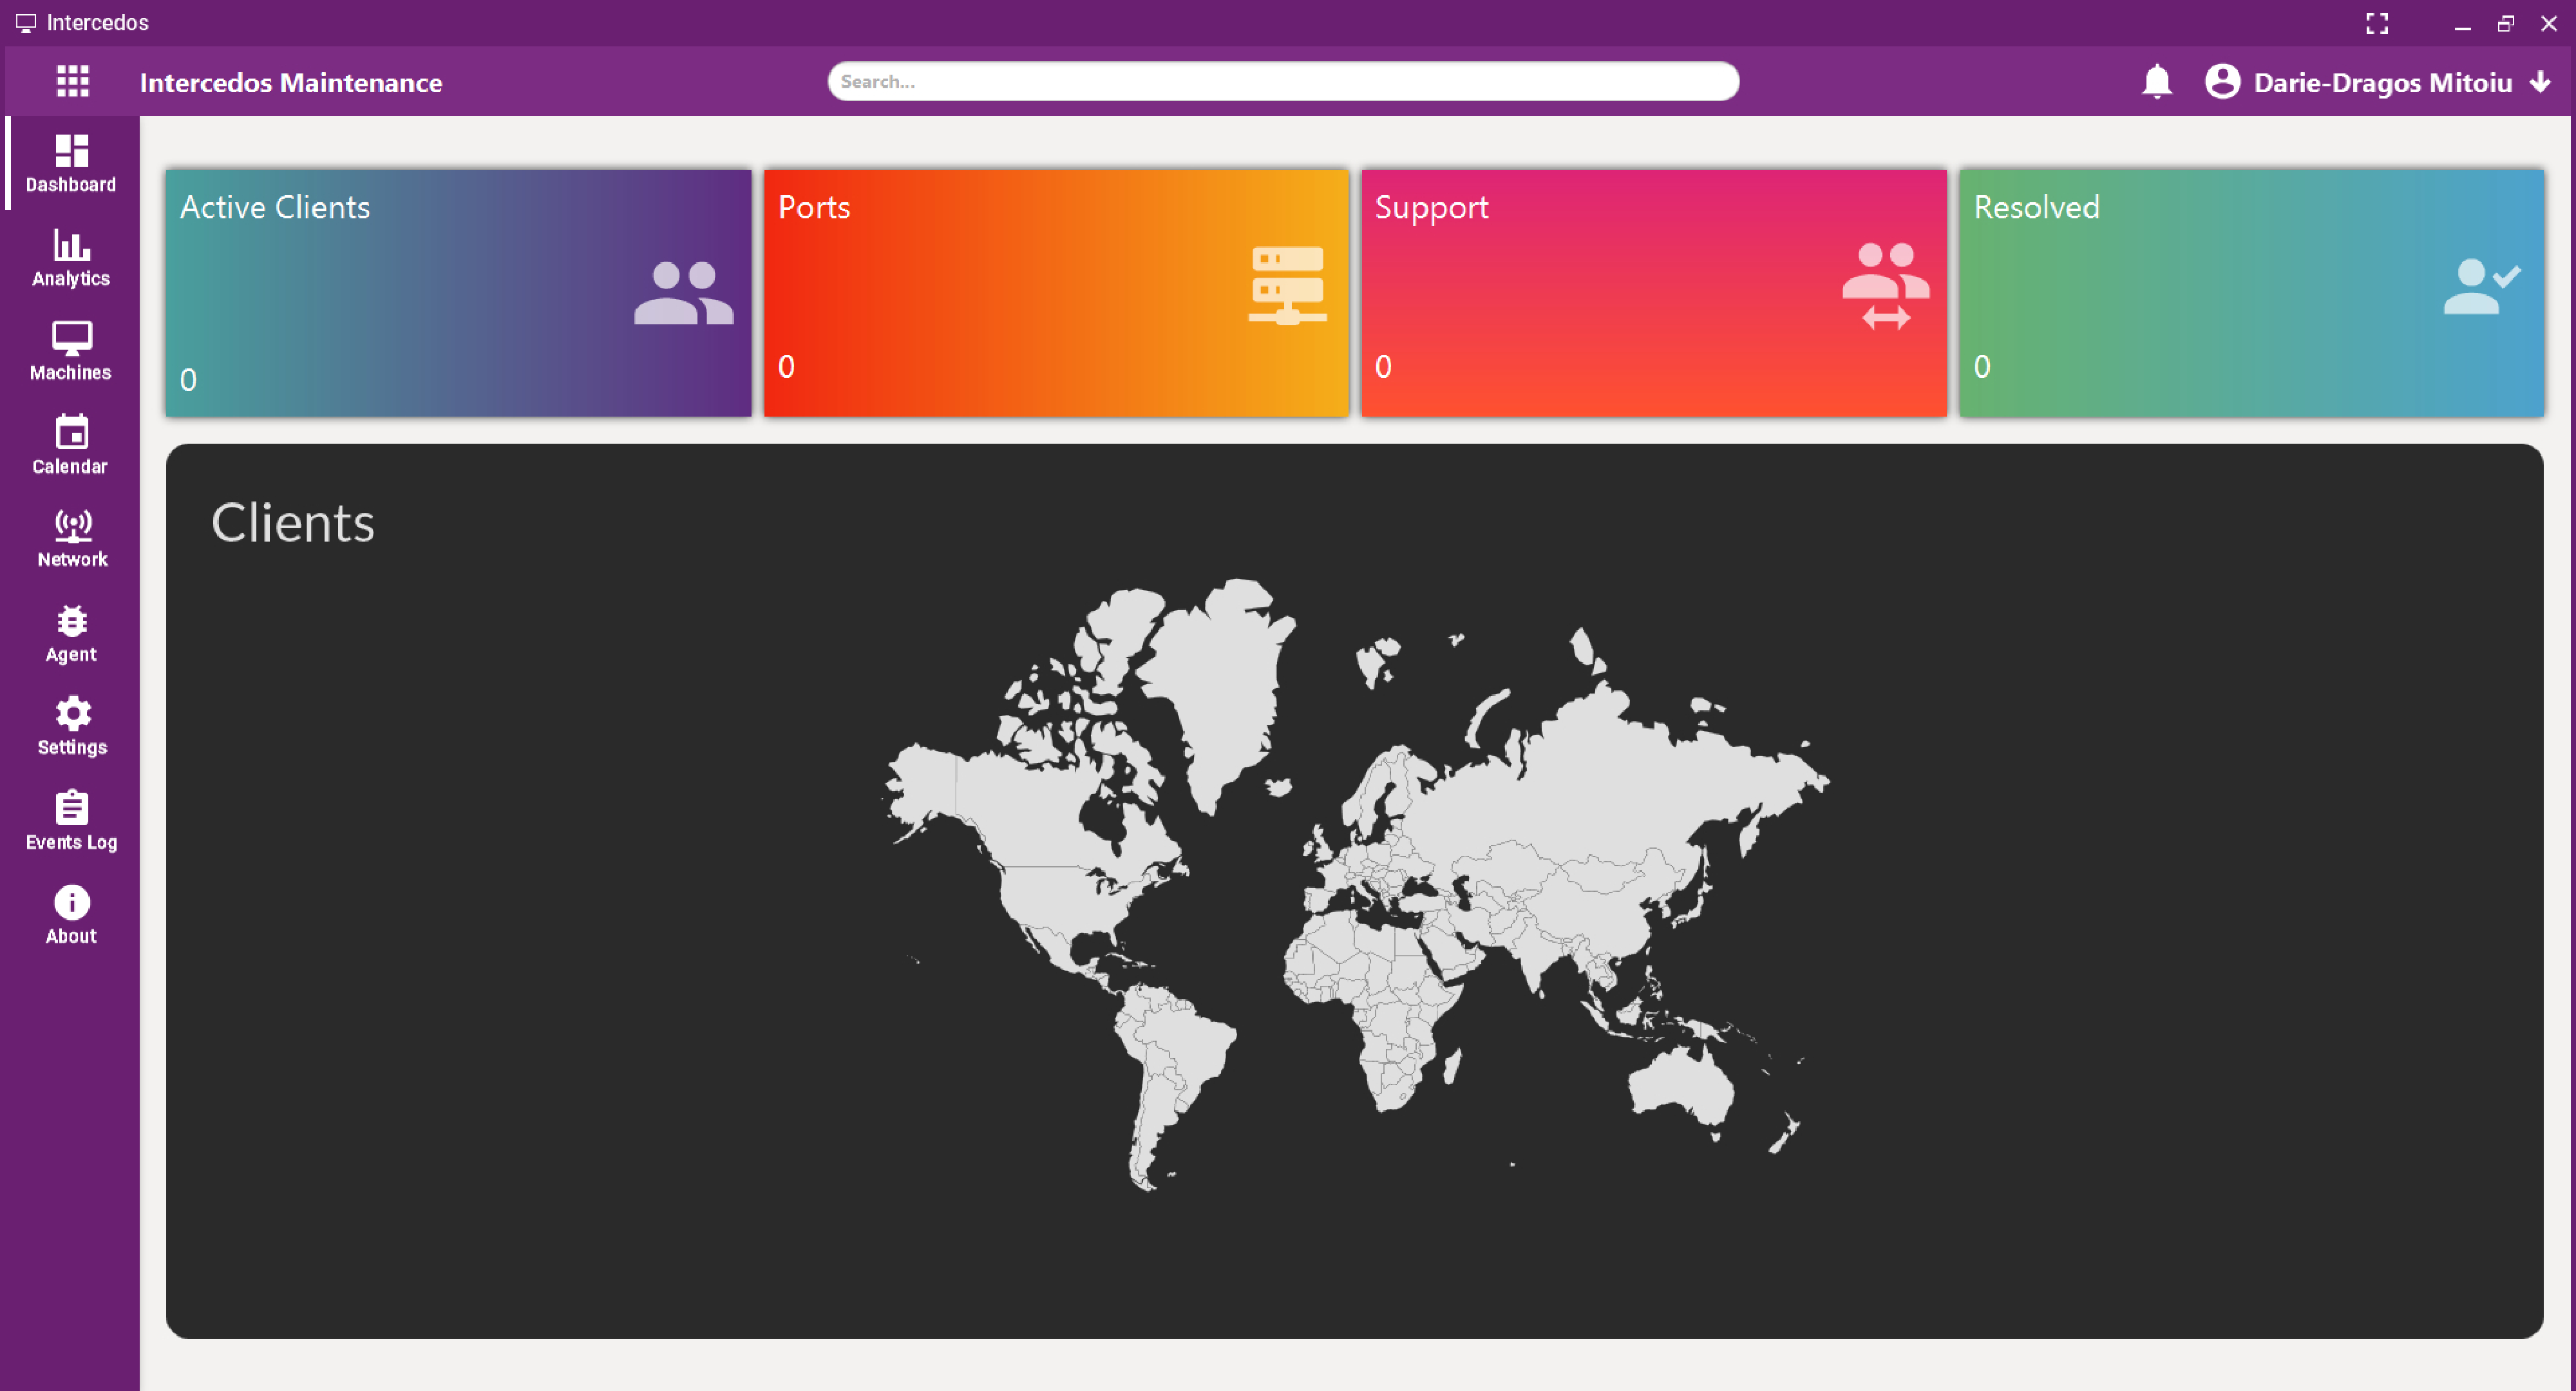
\includegraphics[width=1.0\textwidth]{images/dashboard-light-theme.pdf}
    \captionsetup{justification=centering}
    \caption[Command and Control (C\&C) Light Theme]{Command and Control (C\&C) Light Theme}
    \label{fig:command-light-theme}
\end{figure}

\begin{figure}[h]
    \centering
    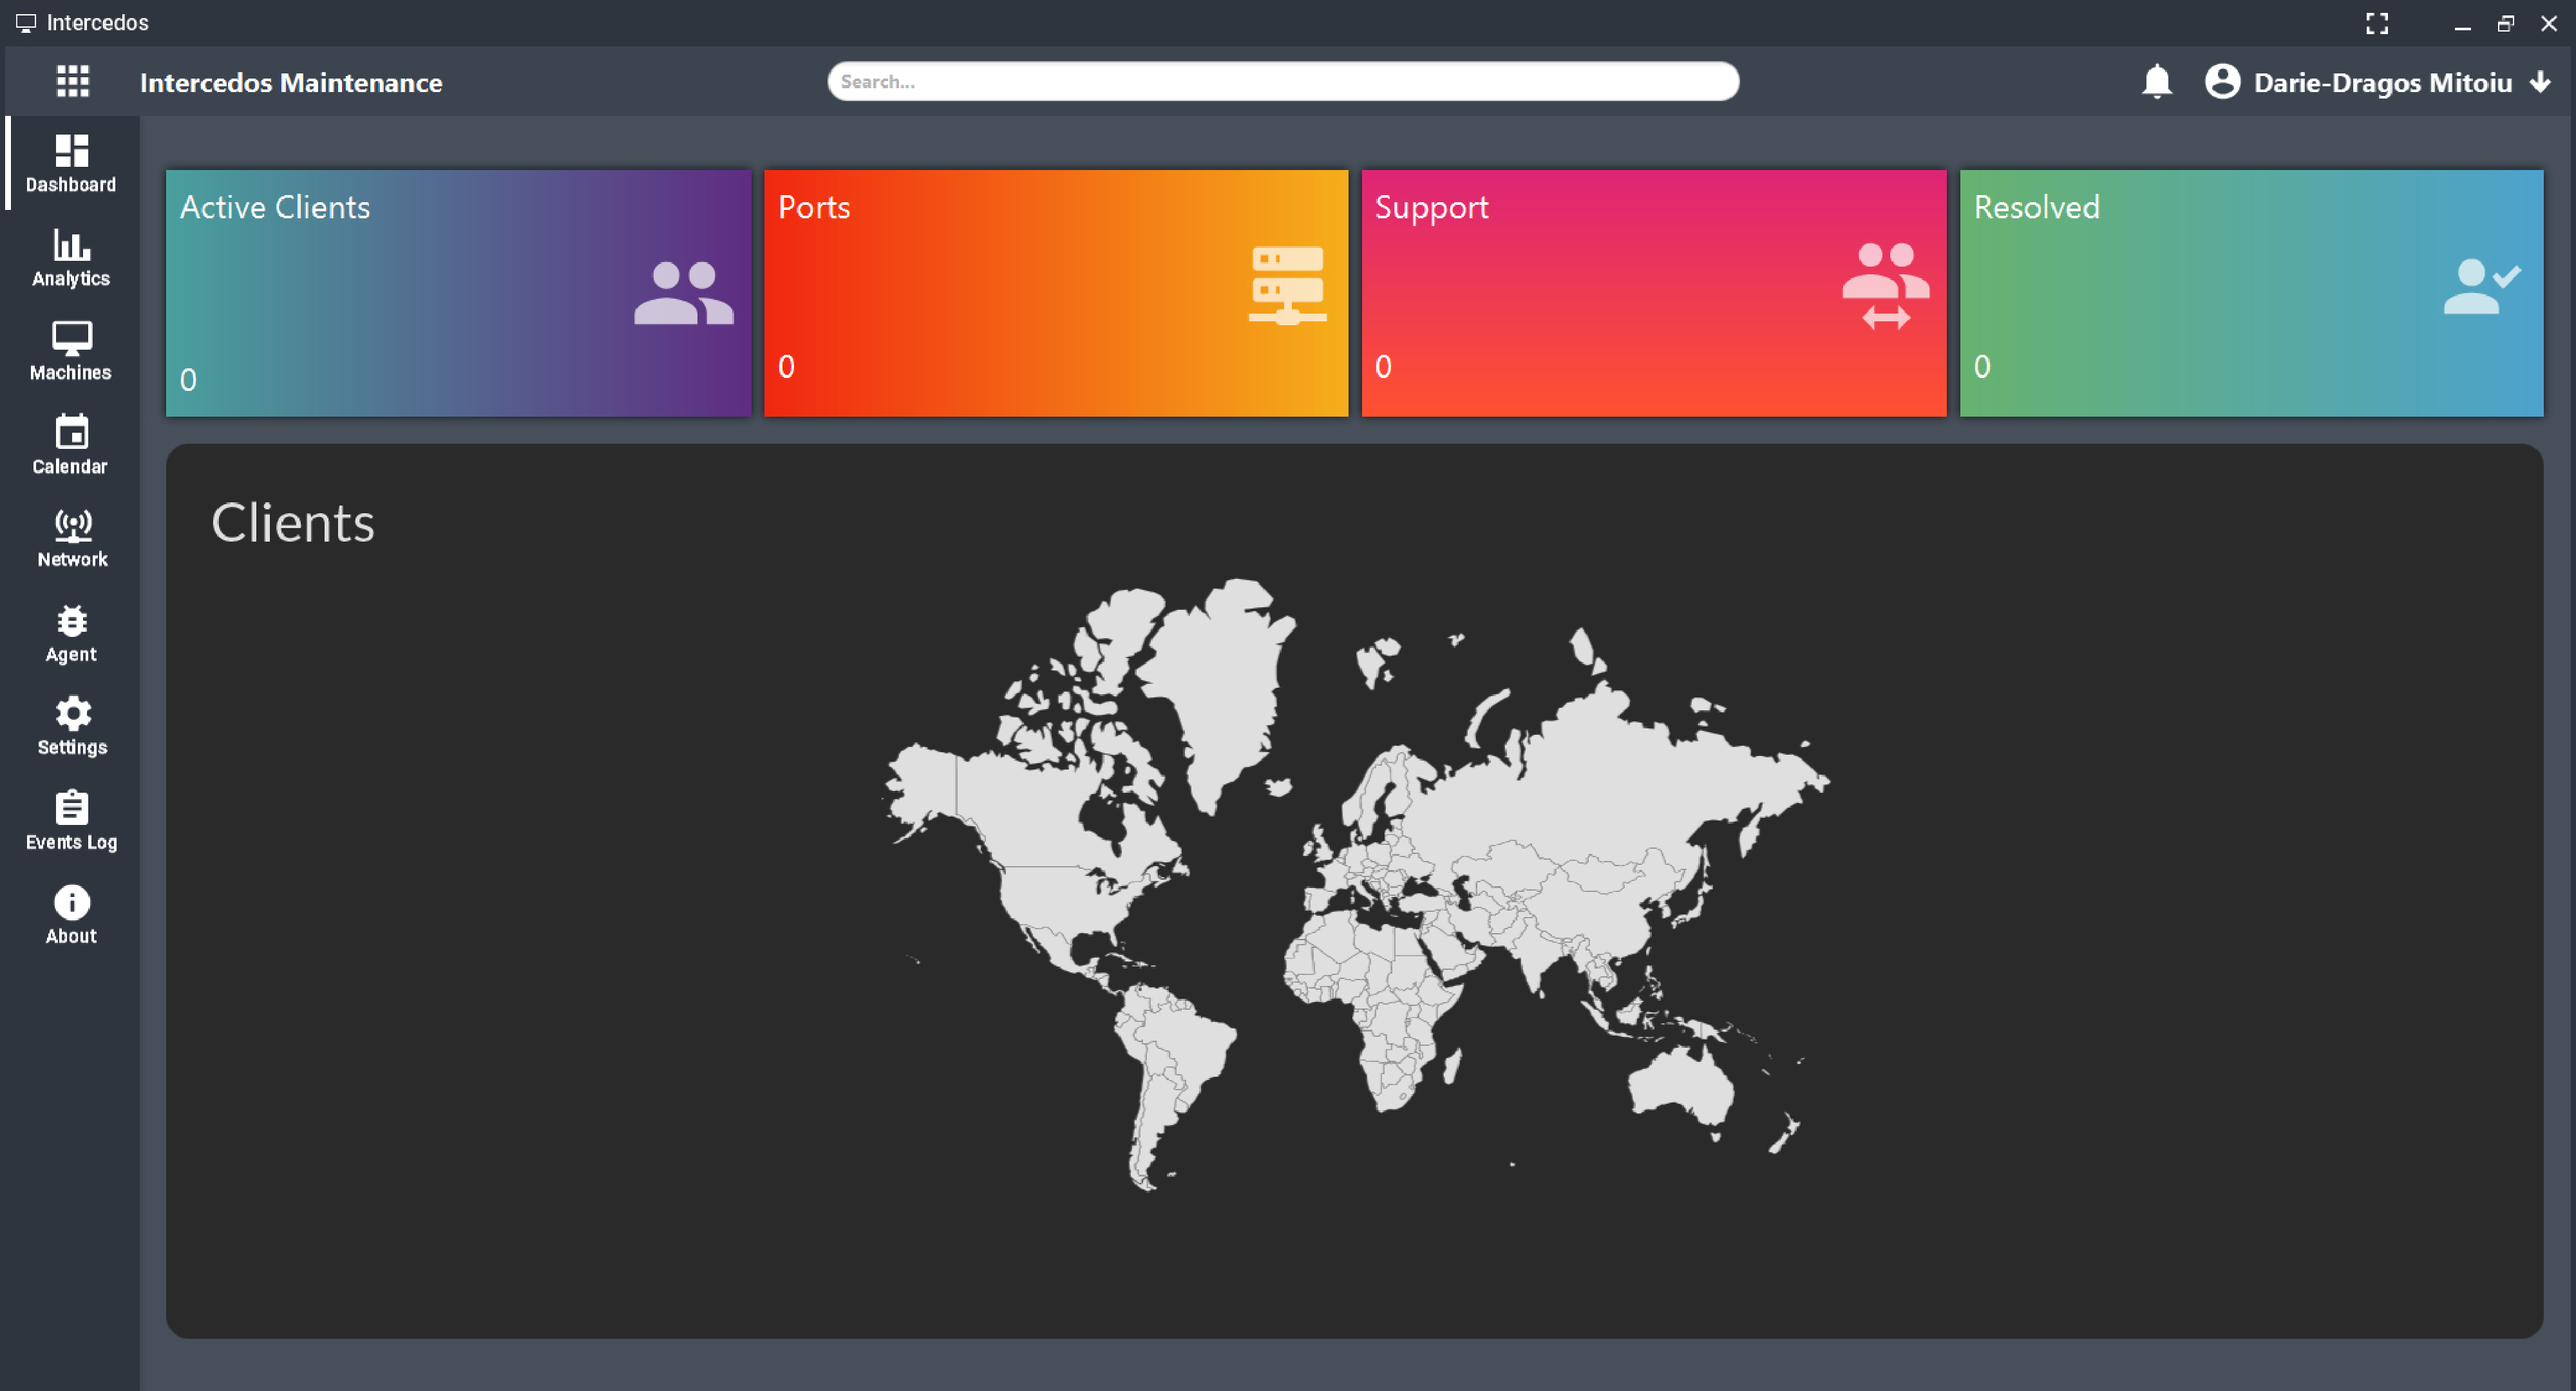
\includegraphics[width=1.0\textwidth]{images/dashboard-dark-theme.pdf}
    \captionsetup{justification=centering}
    \caption[Command and Control (C\&C) Dark Theme]{Command and Control (C\&C) Dark Theme}
    \label{fig:command-dark-theme}
\end{figure}

\newpage

\begin{figure}[h]
    \centering
    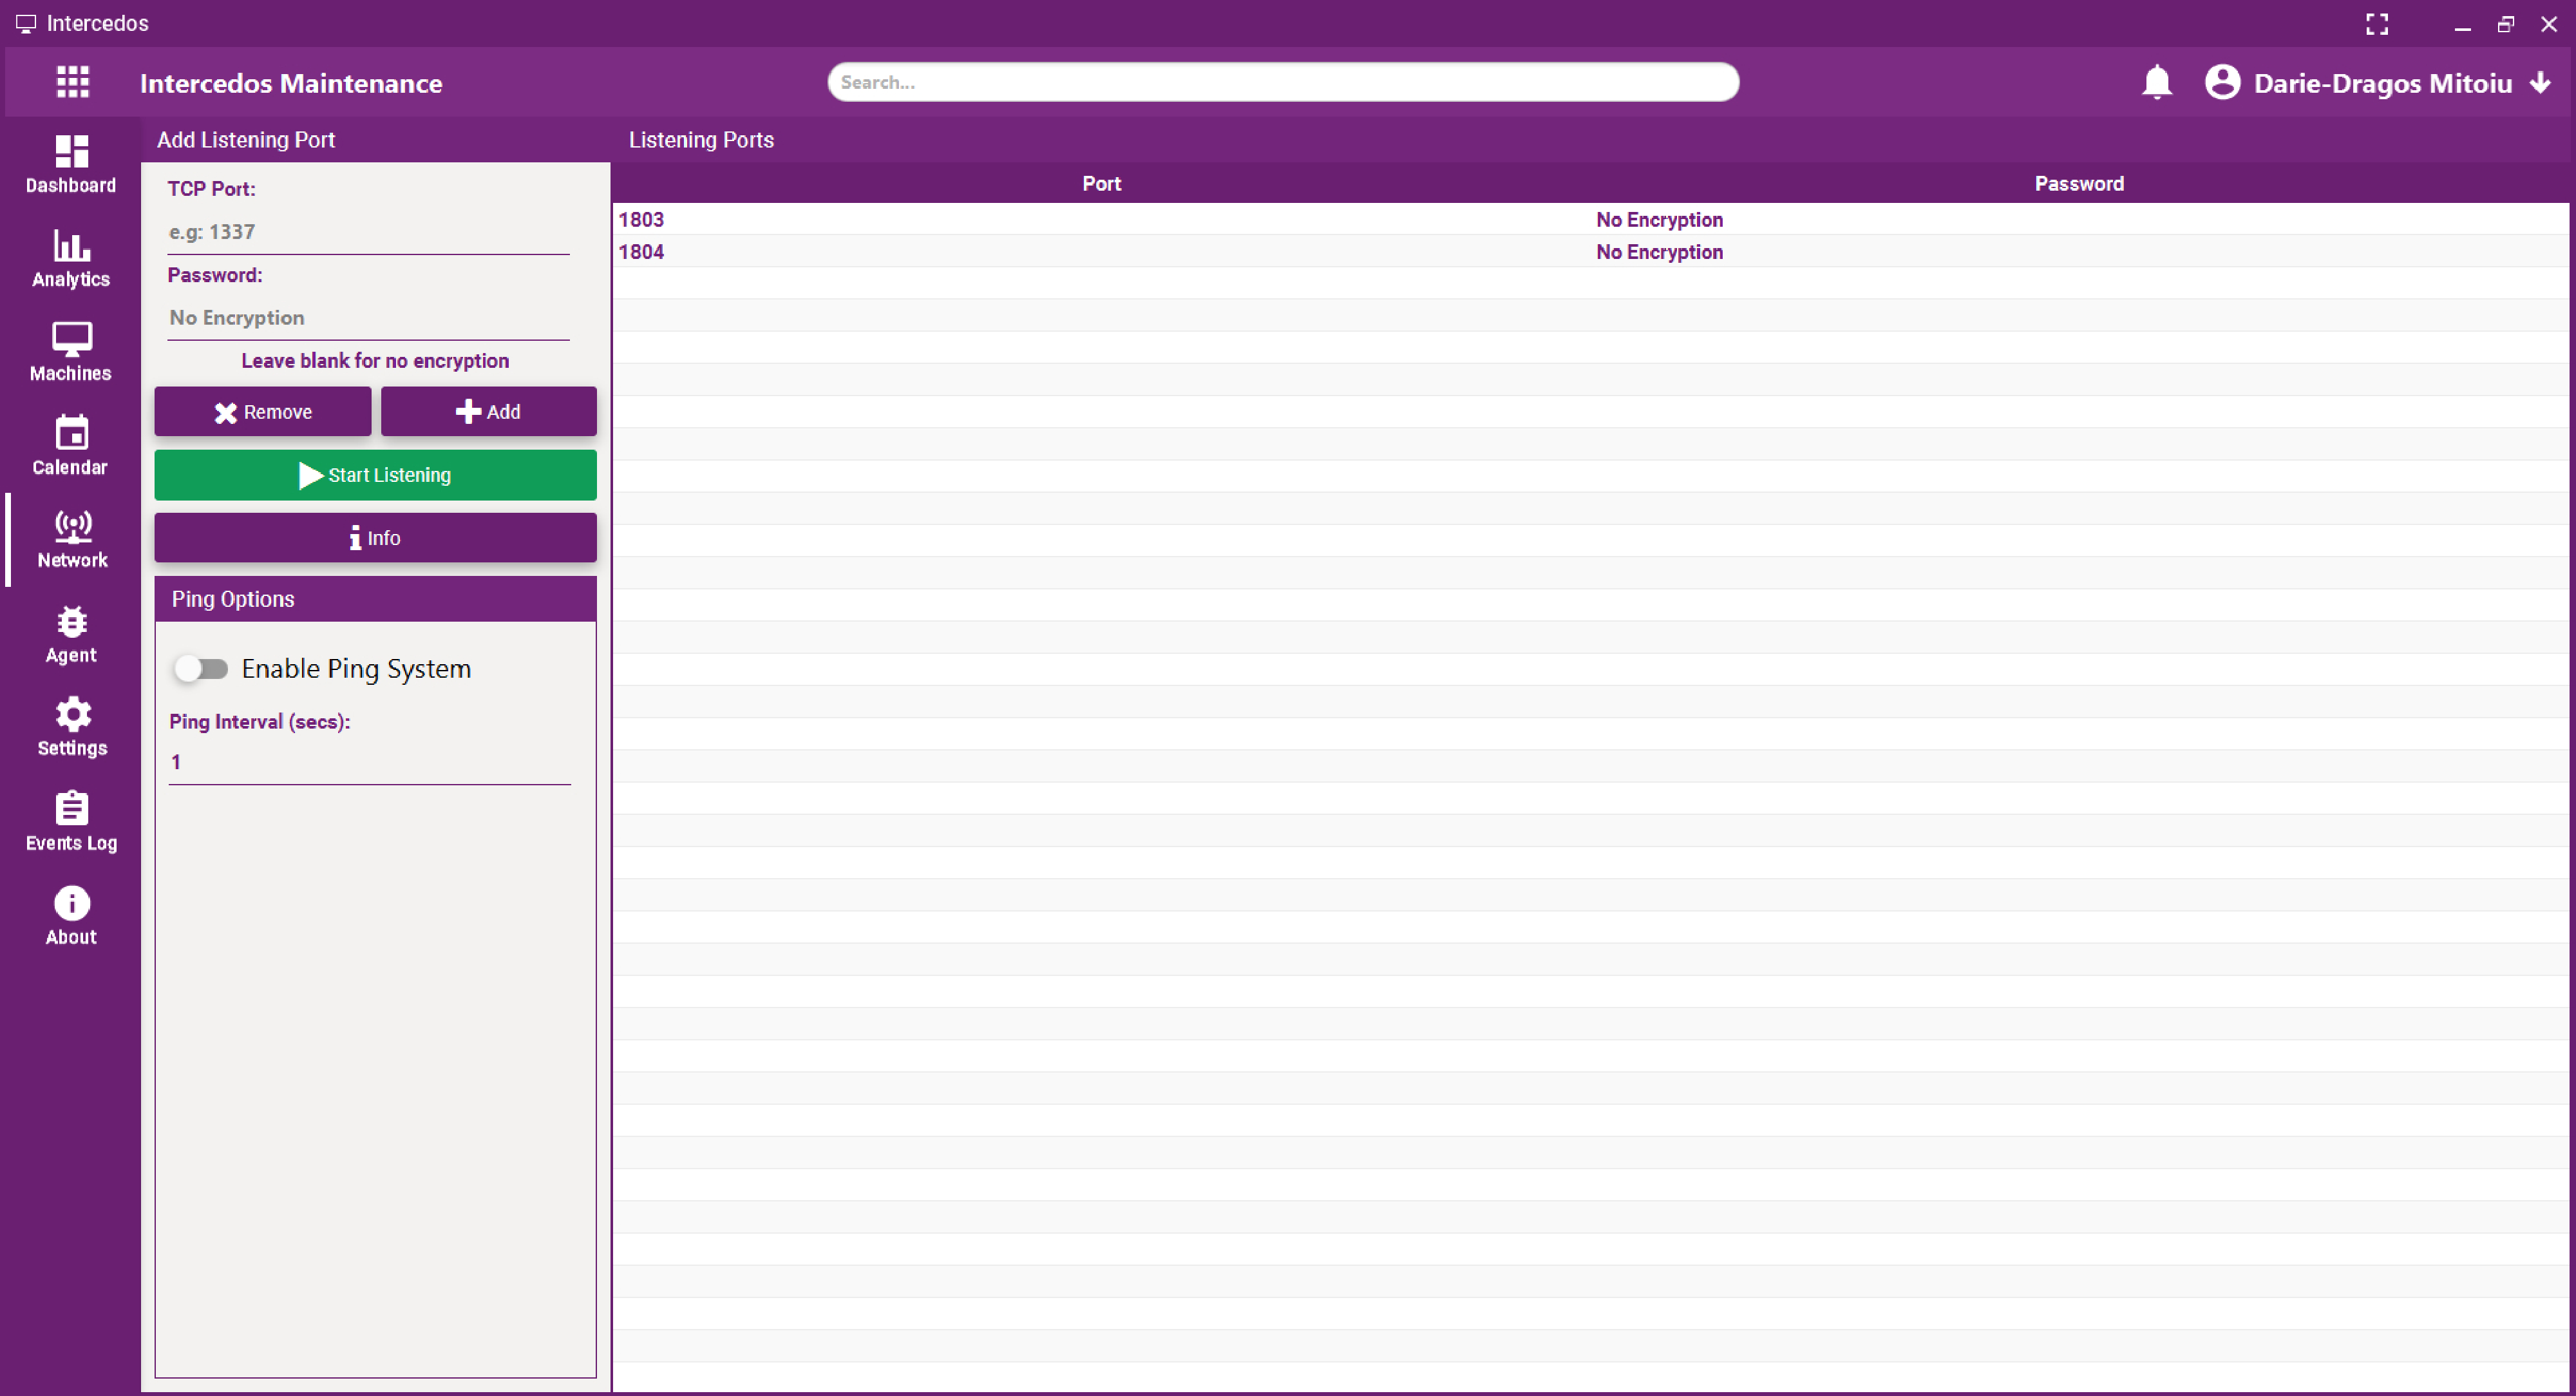
\includegraphics[width=1.0\textwidth]{images/network-panel-light-theme.pdf}
    \captionsetup{justification=centering}
    \caption[Command and Control (C\&C) Network Panel]{Command and Control (C\&C) Network Panel}
    \label{fig:command-network}
\end{figure}

\begin{figure}[h]
    \centering
    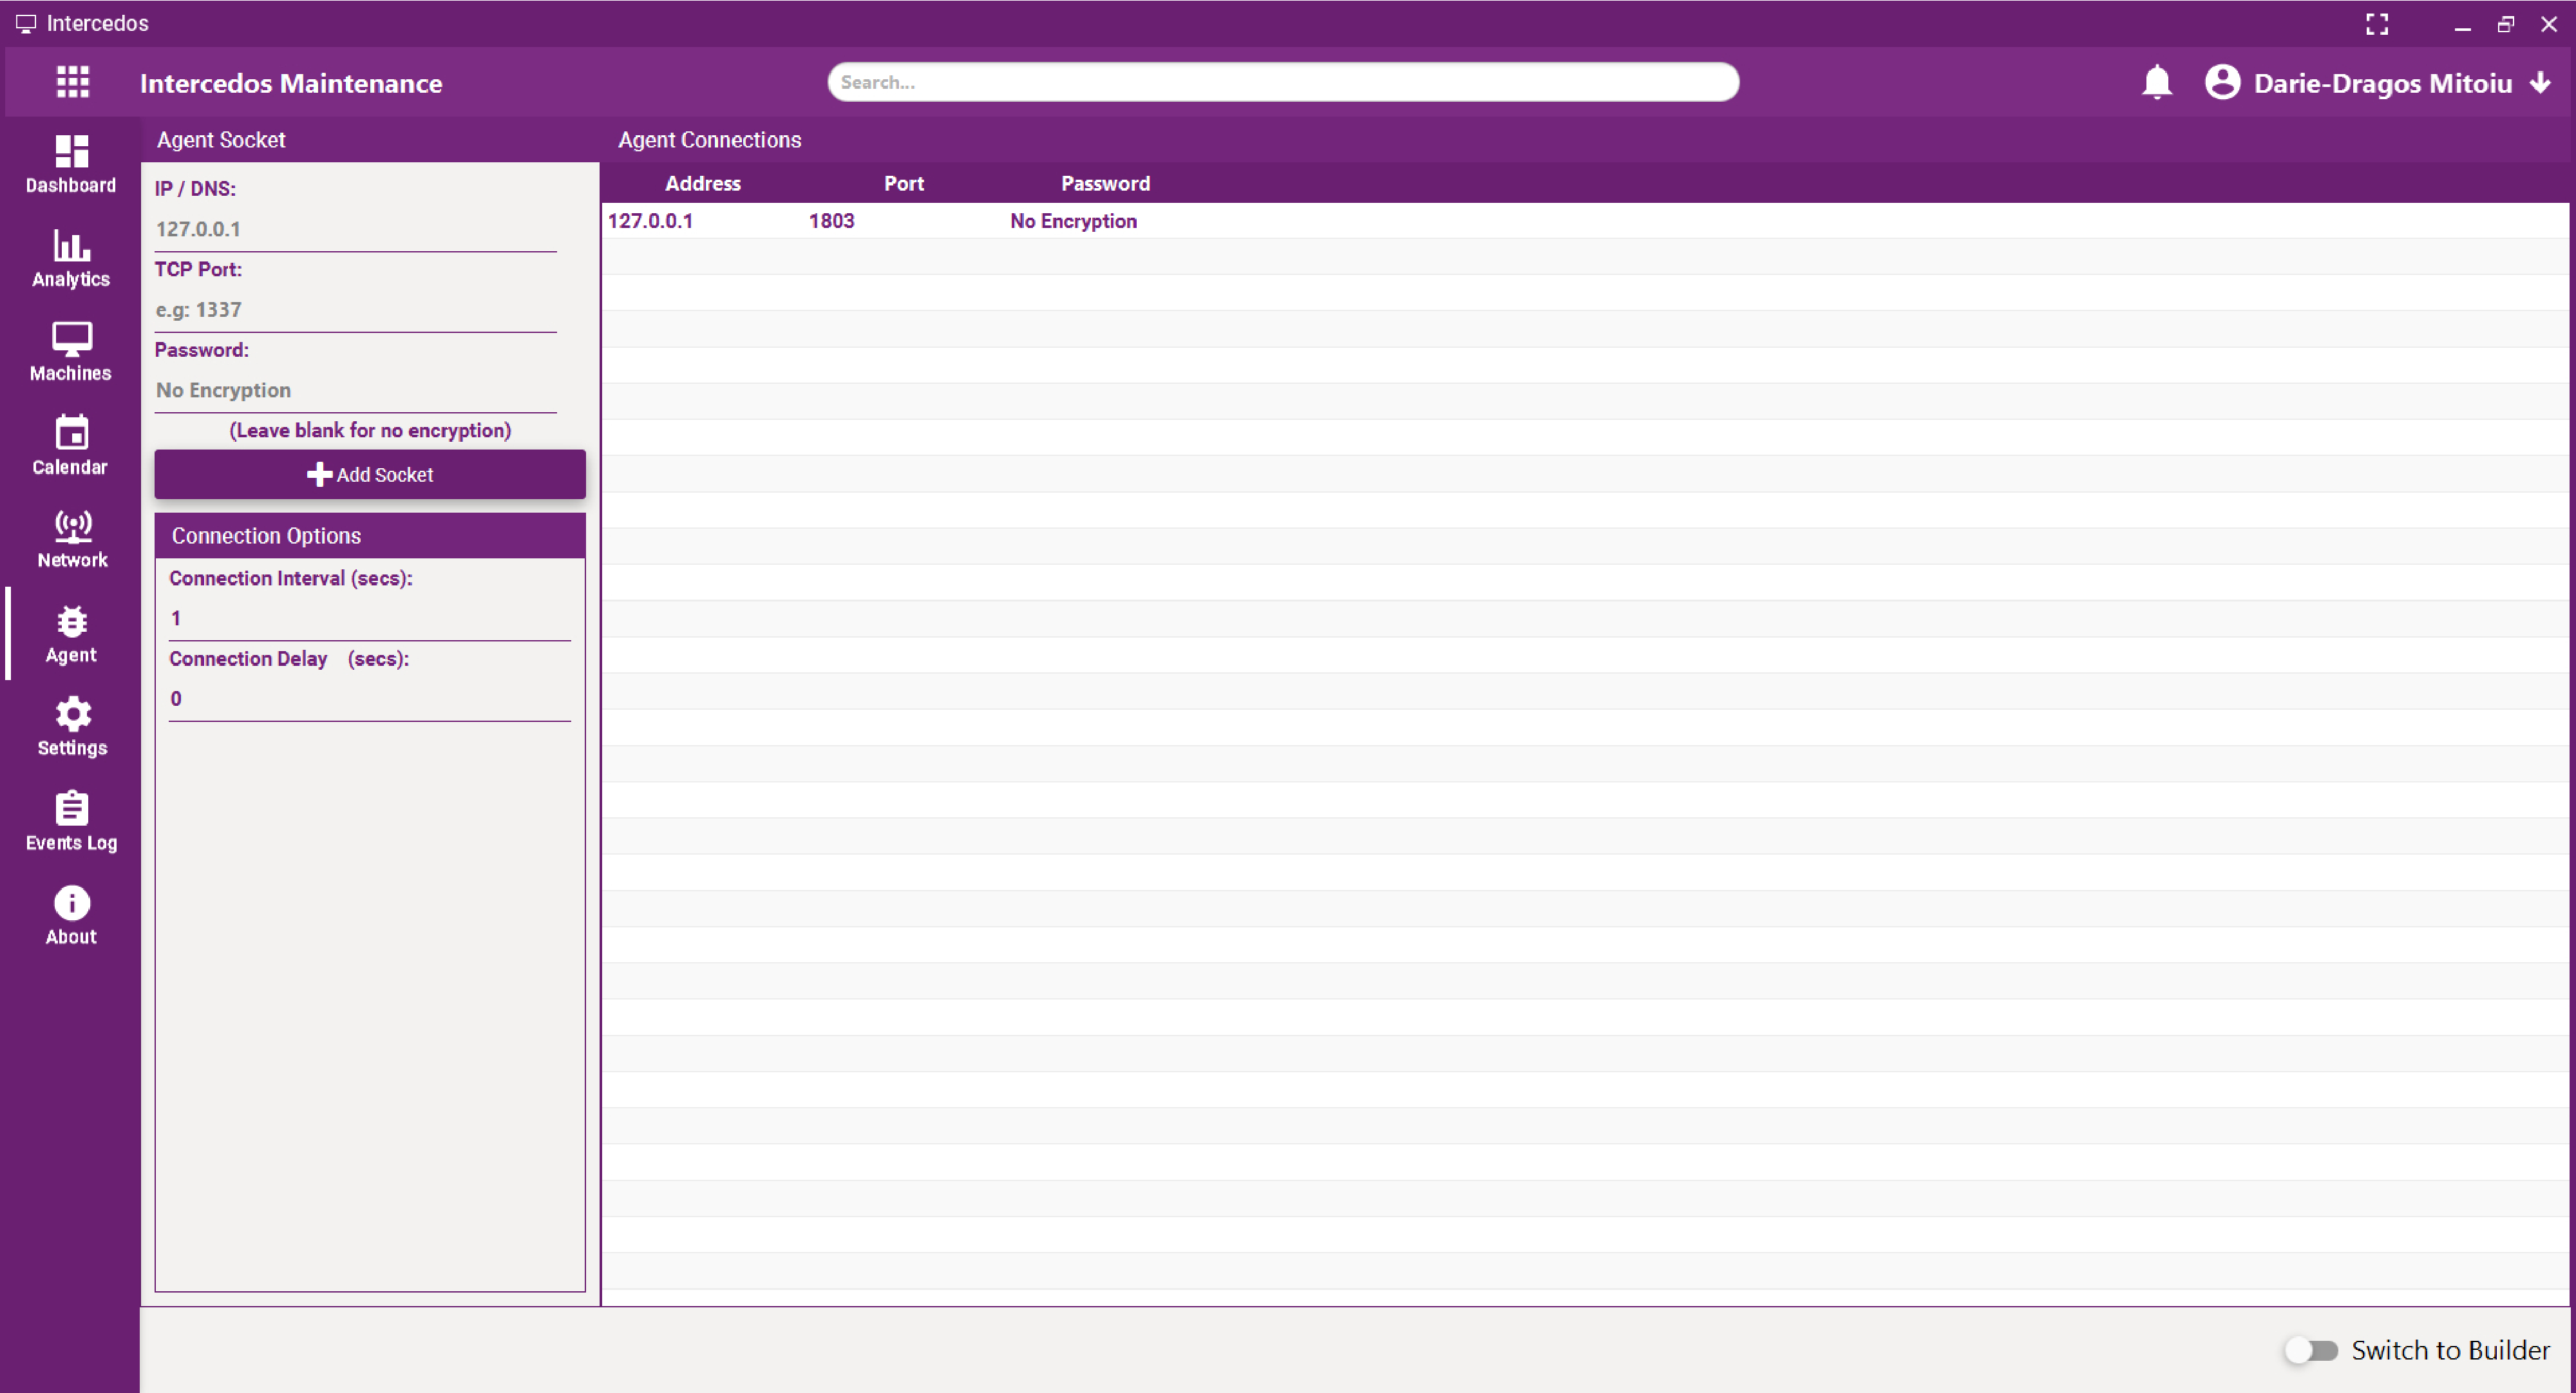
\includegraphics[width=1.0\textwidth]{images/agent-panel-light-theme.pdf}
    \captionsetup{justification=centering}
    \caption[Command and Control (C\&C) Agent Panel]{Command and Control (C\&C) Agent Panel}
    \label{fig:command-agent}
\end{figure}

\newpage

\subsubsection{MigLayout}

The creation of rich and complex Graphical User Interfaces can be a tedious and time
consuming process. Both Swing and JavaFX Interface Frameworks present build-in containers
or layouts which will allow the creation of the graphical user interface either by writing
Java instructions or just by using a third-party tool such as Scene Builder for JavaFX
which will generate some FXML based on some interactions with a graphical
user interface tool. However, this process is not efficient enough as even with the help of
third-party tool such as Scene Builder in the case of JavaFX as there will still
be limitations in the graphical user interface created without some additions of multiple
types of layouts to create the desired result, as the build-in layouts lack the capabilities to create
rich and complex layouts using just a single type of layout. This problem it is addressed
by the third-party layout called MigLayout which it is a grid based type of layout designed
specifically to avoid the utilisation of multiple types of containers or layouts to achieve
the desired result, the MigLayout container can be used for both Swing Interface Framework
and the JavaFX Interface Framework with the same syntax achieving the same result.
The \acrfull{cc} Server Application has been built using mostly the MigLayout for the
creation of the application's containers, this layouts has allowed the acceleration of
the development of the application in a significant way due to the numerous features
randing from the creation of responsive Graphical User Interfaces to the ability to
add or remove graphical components at need during run-time of the application.
It must be noted that each Graphical User Interface, Swing or JavaFX, will require
a different type of MigLayout dependency in order to function properly,
the interoperability will still be possible with the use of the MigLayout between
the Swing Framework and the JavaFX Framework, yet the appropriate Interface Nodes
must be used.

\subsection{Controller}

The controller of the \acrfull{cc} Server application will have the role to act as an
intermediary between the Graphical User Interface (JavaFX) and the models of the
application. As composition, the controller will consists of a package called
authentication, database, network, messages, build and logger. The authentication
package will contain Java Classes related to the Amazon Cognito Authentication Database
for actions such as user registration, user log in and password recovery. The database
package will contain Java Classes related to the local SQLite Database which will hold
specific ports which can be opened by the \acrfull{cc} Server. The network package will
hold packages related to the networking programming aspect of the application such as
the TCP Server with the associated Object Input Stream and Object Output Stream for data
transmission. The messages package will contain Java Classes related to specific Java
Classes which will behave as network packets as all classes in this package implement the
Serializable Java Interface. The Build package will contain code related to the creation
of the agent application. The logger package will contain Java Classes related to the
appending of informative log events which will be added to the Graphical User Interface.

\newpage
\subsubsection{Agent Configuration}

\begin{lstlisting}[language=Java, label={lst:agent-constants}, style=Oracle, columns=fullflexible,
caption=Agent (Client-Side) Constants Class,
captionpos=b]
public class Constants {
    public final static String SERVER_ADDRESS = "127.0.0.1";
    public final static int SERVER_PORT = 1337;
    public final static String T_CLASS = "/client/ClientApplication.class";
    public final static String T_METHOD = "main";
    public final static String T_DESCRIPTOR = "([Ljava/lang/String;)V";
}
\end{lstlisting}

\begin{lstlisting}[language=Java, style=Oracle, columns=fullflexible,
caption=Agent (Client-Side) Java Bytecode Manipulation,
captionpos=b]
ClassVisitor classVisitor = new ClassVisitor(ASM5, cw) {
    @Override
    public FieldVisitor visitField(int access,String name,String descriptor,
                                   String signature,Object value) {
        if(name.equals("SERVER_ADDRESS"))
            value = serverAddress;
        if(name.equals("SERVER_PORT"))
            value = serverPort;
        return super.visitField(access,name,descriptor,signature,value);
    }
    @Override
    public MethodVisitor visitMethod(int access,String name,String desc,
                                     String signature,String[] exceptions) {
        MethodVisitor mv = super.visitMethod(
                access, name, desc, signature, exceptions);
        if(name.equals(Constants.T_METHOD)
                && desc.equals(Constants.T_DESCRIPTOR)) {
            return new MethodVisitor(Opcodes.ASM5, mv) {
                @Override
                public void visitLdcInsn(Object address) {
                    if(Constants.SERVER_ADDRESS.equals(address))
                        address = serverAddress;
                    super.visitLdcInsn(cst);
                }
                @Override
                public void visitIntInsn(int i, int port) {
                    if(Constants.SERVER_PORT == port)
                        port = serverPort;
                    super.visitIntInsn(i, port);
                }
            };
        }
        return mv;
    }
};
\end{lstlisting}

\newpage

\begin{lstlisting}[language=Java, label={lst:agent-configuration}, style=Oracle, columns=fullflexible,
caption=Agent (Client-Side) Configuration Creation,
captionpos=b]
private static byte[] createConfiguration(String serverAddress,
                                          int serverPort) {
    log.info("Generating agent configuration...");
    String modifyClass = Constants.T_CLASS;
    InputStream path = Constants.class.getResourceAsStream(modifyClass);
    ClassReader cr = new ClassReader(path);
    ClassWriter cw = new ClassWriter(cr,0);
    cr.accept(classVisitor, 0);
    cw.visitEnd();
    return cw.toByteArray();
}
\end{lstlisting}

The \acrfull{cc} Server Application will present a feature which can be considered to be at
the core of the application when it comes to the Hard-Disk Drive \acrfull{smart} indicators
data retrieval, this feature is the agent creation which it is one of the most complex
features of the application as it involves the manipulation of Java Bytecode in order
ratify a series of instructions due to the dynamic configuration of the agent by the
user using the Graphical User Interface. In the figure \ref{lst:agent-constants}
it can be observed a list of static constants which have the role to hold the agent
configuration and the Java Class Manipulation Key values. The constants are placed
into a class called "Constants" which will allow the access to these values by calling
the "Constants" class though the project. The constants called "SERVER\_ADDRESS" refers
to the IP address which will be given to the agent application dynamically by the \acrfull{cc}
application in order to establish a connection, usually this address would be the same
address of the machine which will execute or run the \acrfull{cc} Server Application.
The constant called "SERVER\_PORT" refers to the port given to the agent application
dynamically by the \acrfull{cc} application to complement the previous IP address.
The "Constants" Class also contains a series of constants which are aiming at the
Java Bytecode manipulation of a specific Java Class, these constants use the prefix letter
"T" which stands for transform, the contant class called "T\_CLASS" specifies the class
to be modified at run-time, the constant called "T\_METHOD" specifies the method which
has to be modified at run-time and last but not the least the constant called
"T\_DESCRIPTOR" it is used in order to specify the type of the method which will be
modified which in this case it is a String type. The transform constants will be used
in association with the ClassVisitor of the ASM Java Bytecode Manipulation Library from
France Telecom. The ClassVisitor object created will perform all the modifications required
based on the transform constants. Once the classVisitor object it is created then the
generation of the agent configuration can happen as it can be seen in
the \ref{lst:agent-configuration} and the newly created class it is
returned from the method as a byte array which will be used at
the creation of the Java Archive (.jar).
The constants and variables used in the \ref{lst:agent-constants} code list and
\ref{lst:agent-configuration} code list have been adapted in order to fit in the
paper of the document, to explain the shorthands used in the naming of the
constants.

\newpage

\subsubsection{Agent Builder}

\begin{lstlisting}[language=Java, style=Oracle, columns=fullflexible,
caption=Agent (Client-Side) Builder,
captionpos=b]
private static void jarBuilder(File input, File output){
    try{
        JarFile jarFile = new JarFile(input);
        String className = ClientApplication.class.getName();
        String clientClass = "client/controller/network/Constants.class";
        Manifest manifest = new Manifest(jarFile.getManifest());
        manifest.getMainAttributes().putValue("Main-Class", className);

        FileOutputStream fileOutStream;
        JarOutputStream jarOutStream;
        fileOutStream = new FileOutputStream(output);
        jarOutSream = new JarOutputStream(fileOutSream, manifest);

        Enumeration<JarEntry> entries = jarFile.entries();
        Host host = (Host) connectionsTable.getItems().get(0);
        byte[] constants = createConfiguration(host.getAddress(),
                                               host.getPort());
        while(entries.hasMoreElements()){
            JarEntry jarEntry = entries.nextElement();
            if(!jarEntry.getName().equals("META-INF/MANIFEST.MF")){
                if(jarEntry.getName().equals(clientClass)){
                    ZipEntry conEntry = new ZipEntry(jarEntry.getName());
                    constantsEntry.setSize(constants.length);
                    jarOutputStream.putNextEntry(conEntry);
                } else {
                    jarOutputStream.putNextEntry(jarEntry);
                }
                if(!jarEntry.isDirectory()){
                    if(jarEntry.getName().equals(clientCLass)){
                        jarOutputStream.write(constants);
                    } else {
                        jarOutputStream.write(IOUtils.
                        toByteArray(jarFile.getInputStream(jarEntry)));
                    }
                }
                jarOutputStream.closeEntry();
            }
        }
        jarFile.close();
        jarOutputStream.close();
    } catch (IOException e){
        e.printStackTrace();
    }
}
\end{lstlisting}

\newpage

\subsection{Authentication System}

The \acrfull{cc} Server Application uses the Amazon Cognito Database in order to grant
access to the main features of the application. The Amazon Cognito Database provides
authentication, authorization and user management for web application, mobile applications
and desktop application. This type of database will allow the user to log in using
their email and password. The two main component of the Amazon Cognito Database are
the User Pools and the Identity pools, the User Pools can be considered as user
directories which can provide registration options for the application, while the
identity pools allow access to other Amazon Services. The Amazon Cognito Database
will require the following fields to be provided by the user in order to allow
the account creation: Given Name, Family Name, Email and Password.

\subsection{Local Database}

The \acrfull{cc} Server Application uses two main SQLite tables, these tables are
the "connections" table and the "banlist" table. The connections table will contain
the ports associated with their passwords which can be seen in the figure
\ref{fig:command-network}. The table called "banlist" does not present any implemented
features in the current version of the \acrfull{cc} Server. However, the "banlist" table
will be used to block specific agent connections at need by using their IP address.

\subsubsection{SQLite Structure}

\begin{lstlisting}[language=SQL, style=Oracle, columns=fullflexible,
       caption=Command \& Control (C\&C) SQLite Tables,
       captionpos=b]
CREATE TABLE connections(
    port integer(10),
    password varchar(255)
);

CREATE TABLE banlist(
    ip varchar(255),
    reason varchar(255)
);
\end{lstlisting}

\begin{lstlisting}[language=SQL, style=Oracle, columns=fullflexible,
caption=Agent (Client-Side) SQLite Tables,
captionpos=b]
CREATE TABLE servers(
    address varchar(255),
    port integer(10),
    description varchar(255),
    password varchar(255)
);
\end{lstlisting}

\subsection{Networking}

\subsubsection{Transmission Control Protocol (TCP)}

The term \acrfull{tcp} refers to the standard method of how to establish and maintain
a network connection or conversation though which applicaions or programs can send
and receive data. The \acrfull{tcp} it is associated with the Internet Protocol (IP)
which defines how computer systems can send packets of data between each other (Lutkevich 2020).

\subsubsection{User Datagram Protocol (UDP)}

The term \acrfull{udp} refers to a protocol of communications that is primarily used for
establishment of connections which are categorised as low-latency and loss-tolerating
connections between applications or programs over the internet. This approach it will
accelerate the transmission of data by enabling the transfer of data before an
agreemenet or hand-shake with the receiving party (Rosencrance and Lawton and Moozakis 2020).

\subsubsection{Hard-Disk Drive S.M.A.R.T Attribute Class}

\begin{lstlisting}[language=Java, style=Oracle, columns=fullflexible,
caption=Hard-Disk Drive S.M.A.R.T Attribute Class,
captionpos=b]
public class DiskAttribute implements Serializable {
    private int id;
    private String name;
    private String flag;
    private int value;
    private int worst;
    private int thresh;
    private String type;
    private String updated;
    private String failed;
    private String raw;

    public DiskAttribute(String name, String flag, int value, int worst,
                         int thresh, String type, String updated,
                         String failed, String raw){
        this.name = name;
        this.flag = flag;
        this.value = value;
        this.worst = worst;
        this.thresh = thresh;
        this.type = type;
        this.updated = updated;
        this.failed = failed;
        this.raw = raw;
    }
}
\end{lstlisting}

\newpage

\section{Agent (Client-Side)}

The Agent (Client-Side) Application it is composed of two main components, these two components
are the controller of the application and the data models which the application is using.
The controller of the application it is split into another two components which the configuration
component and the network component.

\subsection{Controller}

The most important component of the Agent (Client-Side)
application it is the network component as it contains all the necessary tools in order to
retrieve the Hard-Disk Drive \acrfull{smart} indicators data, yet in order to do this, the
agent application must be executed as administrator with the third-party application called
Smartmontools installed on the machine which will run the application.

\subsection{Networking}

The Agent (Client-Side) Application it uses the \acrfull{tcp} in order to communicate with the \acrfull{cc} Server
Application, this is due to the ensurance of the packets tranmission over the network which the \acrfull{tcp}
provides, this aspect is not present for the \acrfull{udp} alternative.

\section{Security}

When it comes to the security of the \acrfull{cc} Server Application and the Agent (Client-Side) Application,
the specifications and design have considered the security concerns related to the transmission of Hard-Disk Drive
\acrfull{smart} data over the network, this consideration can be seen in the figure \ref{fig:command-network}
and figure \ref{fig:command-agent} as the "password" element implies some consideration of symmetric encryption
for the data transfer. However due to lack of time, the current versions of \acrfull{cc} Server Application and
Agent (Client-Side) Application do not present any encryption capabilities and the data is sent unencrypted over
the network.

\section{Testing}

Both \acrfull{cc} Server Application and Agent (Client-Side) have been tested using a manual testing approach, the
results can be seen in the table \ref{table:command-tests} and respectively table \ref{table:agent-tests}. The tables
mentioned do not contain any evidence of the tests, for this aspect the Demonstration of the project will evidence that.

\newpage

\section{Machine Learning}

\subsection{Hard-Disk S.M.A.R.T Indicators}

\noindent
\begin{longtable}{
|p{\dimexpr.40\linewidth-2\tabcolsep-1.3333\arrayrulewidth}% column 1
|p{\dimexpr.60\linewidth-2\tabcolsep-1.3333\arrayrulewidth}|% column 2
}
    \hline
    \centering S.M.A.R.T Attribute ID  & \centering\arraybackslash S.M.A.R.T Attribute Name    \hline
    SMART 1                               & \centering Raw Read Error Rate                     \hline
    SMART 3                               & \centering Spin Up Time                            \hline
    SMART 4                               & \centering Start Stop Count                        \hline
    SMART 5                               & \centering Reallocated Sector Count                \hline
    SMART 7                               & \centering Seek Error Rate                         \hline
    SMART 9                               & \centering Power On Hours                          \hline
    SMART 183                             & \centering Runtime Bad Block                       \hline
    SMART 184                             & \centering End-To-End Error                        \hline
    SMART 187                             & \centering Reported Uncorrectable Errors           \hline
    SMART 188                             & \centering Command Timeout                         \hline
    SMART 189                             & \centering High Fly Writes                         \hline
    SMART 190                             & \centering Temperature Difference                  \hline
    SMART 191                             & \centering G-Sense Error Rate                      \hline
    SMART 193                             & \centering Load Cycle Count                        \hline
    SMART 194                             & \centering Temperature Celsius                     \hline
    SMART 197                             & \centering Current Pending Sector                  \hline
    SMART 198                             & \centering Offline Uncorrectable                   \hline
    SMART 199                             & \centering UDMA CRC Error Count                    \hline
    SMART 200                             & \centering Multi Zone Error Rate                   \hline
    SMART 201                             & \centering Soft Read Error Rate                    \hline
    SMART 202                             & \centering Data Address Mark Errors                \hline
    SMART 203                             & \centering Run Out Cancel                          \hline
    SMART 204                             & \centering Soft ECC Correction                     \hline
    SMART 205                             & \centering Thermal Asperity Rate                   \hline
    SMART 206                             & \centering Flying Height                           \hline
    SMART 207                             & \centering Spin High Current                       \hline
\end{longtable}
\captionof{table}{SMART Attributes Names}

\newpage

\noindent
\begin{longtable}{
|p{\dimexpr.30\linewidth-2\tabcolsep-1.3333\arrayrulewidth}% column 1
|p{\dimexpr.32\linewidth-2\tabcolsep-1.3333\arrayrulewidth}% column 2
|p{\dimexpr.38\linewidth-2\tabcolsep-1.3333\arrayrulewidth}|% column 3
}
    \hline
    \centering S.M.A.R.T Attribute  & \centering Seagate ST4000DM000 & \centering\arraybackslash Hitachi HDS722020ALA330  \\ \hline
    smart\_1\_norm                               & \centering 23\%        & \centering 28\%        \hline
    smart\_1\_raw                                & \centering 2\%         & \centering 15\%        \hline
    smart\_5\_norm                               & \centering 2\%         & \centering 22\%        \hline
    smart\_5\_raw                                & \centering 19\%        & \centering 31\%        \hline
    smart\_7\_norm                               & \centering 14\%        & \centering -           \hline
    smart\_7\_raw                                & \centering 26\%        & \centering -           \hline
    smart\_183\_norm                             & \centering 0.5\%       & \centering -           \hline
    smart\_183\_raw                              & \centering 0.5\%       & \centering -           \hline
    smart\_184\_norm                             & \centering 1\%         & \centering -           \hline
    smart\_184\_raw                              & \centering 1\%         & \centering -           \hline
    smart\_187\_norm                             & \centering 21\%        & \centering -           \hline
    smart\_187\_raw                              & \centering 21\%        & \centering -           \hline
    smart\_188\_norm                             & \centering 0\%         & \centering -           \hline
    smart\_188\_raw                              & \centering 10\%        & \centering -           \hline
    smart\_189\_norm                             & \centering 1\%         & \centering -           \hline
    smart\_189\_raw                              & \centering 1\%         & \centering -           \hline
    smart\_190\_norm                             & \centering 2\%         & \centering -           \hline
    smart\_190\_raw                              & \centering 2\%         & \centering -           \hline
    smart\_193\_norm                             & \centering 10\%        & \centering -           \hline
    smart\_193\_raw                              & \centering 63\%        & \centering -           \hline
    smart\_194\_norm                             & \centering 2\%         & \centering 31\%        \hline
    smart\_194\_raw                              & \centering 2\%         & \centering 2\%         \hline
    smart\_197\_norm                             & \centering 5\%         & \centering 4\%         \hline
    smart\_197\_raw                              & \centering 27\%        & \centering 22\%        \hline
    smart\_198\_norm                             & \centering 6\%         & \centering -           \hline
    smart\_198\_raw                              & \centering 27\%        & \centering -           \hline
\end{longtable}
\captionof{table}{SMART Correlation Frequencies for Seagate and Hitachi models
(Botezatu, Giurgiu, Bogojeska and Wiesmann 2016 p. 5 table 2)}

\setlength{\parindent}{1.5em}
\subsection{BackBlaze Data}

In order to prove the viability of forecasting computer systems failure using machine learning techniques and the
Hard-Disk Drive \acrfull{smart} indicators, a series of experiments were performed using data provided by the
BackBlaze company. The Data provided it is from a signle vendor of Hard-Disk componenet which aims at the model
Seagate ST4000DM000, the data also it is relatively new as it is from the year 2017.
This specific study is aiming specifically at the machine learning algorithm
called \acrfull{svm}.

\subsection{Data Exploration}

When the exploration of the data was performed it was seen that the data file contains 142,638 records and 95 features.

\subsection{Data Pre-Processing}

Before creating the machine learning models, a series of pre-processing operations were performed, these
operations are the handling of missing values, the selection of the most relevant features and
the balance of class distribution.

\subsubsection{Features Selection}

According to Beach (2014) the most relevant Hard-Disk Drive \acrfull{smart} features are the following:

\begin{itemize}
    \item SMART 5:   Reallocated\_Sector\_Count,
    \item SMART 187: Reported\_Uncorrectable\_Errors,
    \item SMART 188: Command\_Timeout.
    \item SMART 197: Current\_Pending\_Sector\_Count.
    \item SMART 198: Offline\_Uncorrectable.
\end{itemize}

\subsection{Classification}

\noindent
\begin{longtable}{
|p{\dimexpr.35\linewidth-2\tabcolsep-1.3333\arrayrulewidth}% column 1
|p{\dimexpr.20\linewidth-2\tabcolsep-1.3333\arrayrulewidth}% column 2
|p{\dimexpr.20\linewidth-2\tabcolsep-1.3333\arrayrulewidth}% column 3
|p{\dimexpr.25\linewidth-2\tabcolsep-1.3333\arrayrulewidth}|% column 4
}
    \hline
    \centering Algorithm  & \centering F-1 Score & \centering ROC AUC   & \centering\arraybackslash Accuracy (\%)  \\ \hline
    Support Vector Machines        & \centering 0.44      & \centering 0.67      & \centering 94.56\%        \hline
    Random Forest Model            & \centering 0.50      & \centering 0.70      & \centering 95.10\%        \hline
    Logistic Regression            & \centering 0.45      & \centering 0.68      & \centering 94.61\%        \hline
    Multi-Layer Perceptron         & \centering 0.46      & \centering 0.69      & \centering 94.52\%        \hline
\end{longtable}
\captionof{table}{Best Results for each algorithm used for the experiments}

